\documentclass[sigconf]{acmart}

\usepackage{xspace,framed}
\usepackage{listings}

\setcopyright{acmcopyright}
\acmDOI{10.475/123_4}
\acmISBN{123-4567-24-567/08/06}
\acmConference[EMSOFT '17]{The ACM SIGBED International Conference on Embedded Software }{October 15--20, 2017}{Seoul, South Korea}
\acmYear{2017}
\copyrightyear{2017}
\acmPrice{15.00}


\newcommand\tool{{DSSynth Toolbox}\xspace}

\begin{document}

\title{DSSynth: An Automated Synthesis Tool for Physical Plants \\ Digital Controllers via MATLAB Toolbox}

\begin{abstract}
We present an automated MATLAB Toolbox, named as DSSynth 
(Digital System Synthesis), to synthesize stable and safe digital-control 
systems for physical plants represented as linear time-invariant
systems with single-input and single-output. DSSynth synthesizes digital 
controllers w.r.t. the stability and safety specifications, considering finite word-length 
effects for physical plants represented by transfer-function or state-space 
equations. DSSynth considers fixed-point numerical representation for the 
digital controller and dynamic input ranges for the closed-loop control system. 
Currently, there are two DSSynth toolbox versions: command-line and 
MATLAB application. The resulting toolbox enables application of synthesis to 
real-world systems by control engineers.
\end{abstract}

%
% The code below should be generated by the tool at
% http://dl.acm.org/ccs.cfm
% Please copy and paste the code instead of the example below. 
%
\begin{CCSXML}
<ccs2012>
<concept>
<concept_id>10010520.10010570</concept_id>
<concept_desc>Computer systems organization~Real-time systems</concept_desc>
<concept_significance>500</concept_significance>
</concept>
<concept>
<concept_id>10010520.10010553.10010562</concept_id>
<concept_desc>Computer systems organization~Embedded systems</concept_desc>
<concept_significance>300</concept_significance>
</concept>
<concept>
<concept_id>10011007.10010940.10010992.10010998.10003791</concept_id>
<concept_desc>Software and its engineering~Model checking</concept_desc>
<concept_significance>500</concept_significance>
</concept>
<concept>
<concept_id>10011007.10010940.10010992.10010998</concept_id>
<concept_desc>Software and its engineering~Formal methods</concept_desc>
<concept_significance>100</concept_significance>
</concept>
<concept>
<concept_id>10003752.10003790.10011192</concept_id>
<concept_desc>Theory of computation~Verification by model checking</concept_desc>
<concept_significance>300</concept_significance>
</concept>
</ccs2012>
\end{CCSXML}

\ccsdesc[500]{Computer systems organization~Real-time systems}
\ccsdesc[300]{Computer systems organization~Embedded systems}
\ccsdesc[500]{Software and its engineering~Model checking}
\ccsdesc[100]{Software and its engineering~Formal methods}
\ccsdesc[300]{Theory of computation~Verification by model checking}

\keywords{Formal Synthesis; Digital Control Systems; MATLAB Toolbox; Finite-Word Length; Verification}

\maketitle

%---------------------------------------------------
\section{Introduction}
%---------------------------------------------------

Linear-Time Invariant (LTI) systems are used in several applications
to support non-trivial tasks when applied to embedded systems 
(e.g., robot manipulator, power plants and guidance system). 
In addition, controllers synthesis for LTI systems is richly studied 
by different researchers~\cite{mazo2010pessoa,DBLP:conf/emsoft/RavanbakhshS16,economakos2016automated}; 
however, there are many challenges when 
digital-control systems theory is used due to the finite-word 
length (FWL) effects~\cite{Guang2013, Istepanian2001}, time discretization 
and quantization noise, which are typically introduced by Analogue-to-Digital 
(ADC) and Digital-to-Analogue (DAC) conversion, leading to truncation 
or round-off errors~\cite{astrom1997computer}. 

Embedded digital control systems perform computations over digital signals 
to influence the system behavior~\cite{Ogata2001}; it can be mathematically 
expressed as difference equations, transfer functions or state-space equations. 
Here, the focus is on transfer-function and state-space representations. 
The following expression presents the general form of a digital control system 
using the transfer function representation:
%
\begin{equation}
\small
\label{eq:transferfunction}
H(z)=\frac{B(z)}{A(z)}=\frac{b_{0}+b_{1}z^{-1}+...+b_{M}z^{-M}}{1+a_{1}z^{-1}+...+a_{N}z^{-N}},
\end{equation}
%
\noindent where $z^{-1}$ is called backward-shift operator, $A(z)$ and $B(z)$ are 
the denominator and numerator polynomials, respectively.
%
In state-space format, the digital control system represents the behavior 
of a system via a state evolution equation $\dot{x}(n+1)$ and an instantaneous 
output equation $y(n)$, as follows:
%
\begin{equation}
\begin{split}
\dot{x}(n+1) &= A x(n) + B u(n)
\\
y(n) &= C x(n) + D u(n), 
\end{split}\label{eq:ss-example}
\end{equation}

\noindent where $A$, $B$, $C$ and $D$ are matrices that fully specify a digital system. 

Recently, a new methodology to synthesize digital-control systems was proposed, 
named as DSSynth (Digital System Synthesis)~\cite{abate2017, abatecav2017}, 
which is based on the Counter-Example Guided Inductive Synthesis 
(CEGIS) approach~\cite{DBLP:conf/asplos/Solar-LezamaTBSS06}. Here, CEGIS is used
as a program synthesis engine able to produce controllers for highly non-trivial 
specifications with a very high degree of automation. Program synthesis engines 
as CEGIS use a specification as the starting point, and subsequently 
produce a sequence of candidate programs from a given template. The candidate programs 
are iteratively refined to eventually satisfy the specification. Modern synthesis engines combine 
automated testing, genetic algorithms and SMT-based automated reasoning~\cite{DBLP:journals/corr/AlurFSS16a, DBLP:conf/lpar/DavidKL15}. 
Currently, Abate {\it et al.}~\cite{abate2017} synthesize stable, software-implemented 
embedded controllers, along with a physical plant model represented by transfer functions 
or state-space equations~\cite{abate2017,abatecav2017} using a CEGIS-based approach.

Notably, there are toolboxes in MATLAB with functions and scripts to facilitate the 
digital system design and implementation~\cite{matlab-toolbox}. In fact, there is a MATLAB 
Toolbox named as DSVerifier Toolbox~\cite{issta2017}, which automatically detects 
specific errors related to digital system design ({\it e.g.}, stability, limit cycle and overflow) 
using symbolic model checking techniques based on Boolean Satisfiability (SAT) and 
Satisfiability Modulo Theories (SMT) solvers, given the physical plant and the digital controller. 
However, there is no toolbox in MATLAB to perform digital control synthesis; in particular, based on 
CEGIS considering FWL effects.

The present paper addresses this problem and describes a MATLAB toolbox for DSSynth~\cite{abate2017, abatecav2017} 
in MATLAB's environment named as \tool. The main advantage regarding the use of a MATLAB toolbox 
lies on designing physical plants in MATLAB and then promptly synthesizing a stable digital controller. 
Additionally, when using the \tool, an engineer is able to design a digital system with MATLAB, 
through transfer-function or state-space representations, consider low-level systems parameters 
(implementation features and numerical format), and then gets a stable synthesized digital-controller.

%---------------------------------------------------
\section{Synthesizing Digital Controllers with \tool}
%---------------------------------------------------

%---------------------------------------------------
\subsection{\tool Architecture}
%---------------------------------------------------

The proposed synthesis methodology for closed-loop digital control
systems is based on the DSSynth tool~\cite{abate2017, abatecav2017}, 
which can be split into two main stages as follows: manual (user) and 
automated (DSSynth) procedures, as illustrated in Fig.~\ref{fig:synthesis-flow}. 
%
\begin{figure}[ht!]
\centering
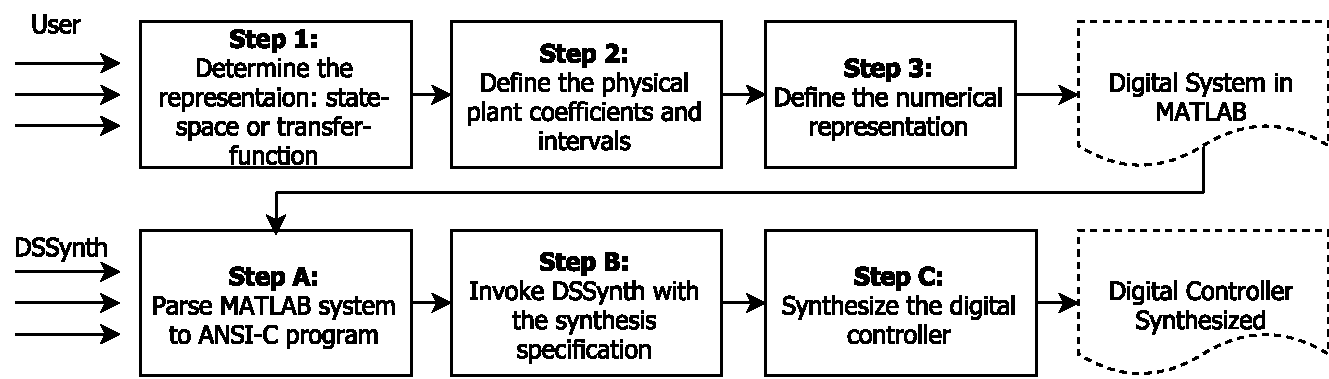
\includegraphics[width=0.45\textwidth]{synthesis-flow.pdf}
\caption{Digital Controller Synthesis Methodology.}
\label{fig:synthesis-flow}
\end{figure}

In step $1$, the user has to define the digital controller representation, 
which can be transfer-function or state-space equations. 
In step $2$, the physical plant (represented by Equations (\ref{eq:transferfunction}) 
and (\ref{eq:ss-example})) must be designed, using the preferred method 
from the control literature~\cite{astrom1997computer}. Finally, in step $3$, 
the numerical representation for the digital controller implementation must be 
defined by the user, {\it i.e.}, the FWL format that includes the number of bits for the integer 
and fractional parts as well as the dynamic range inputs. The result of the manual 
procedure performed by the user is a digital system specification for the given 
physical plant in MATLAB. 

After that, the synthesis process starts in step $A$, when \tool obtains the digital system 
specification in MATLAB, and then translates it into an ANSI-C program. 
In step $B$, our CEGIS engine is invoked to synthesize the digital controller w.r.t. the digital system
specification. Finally, in step $C$, the synthesized digital controller considering FWL effects is produced. 
The output generated by \tool is the synthesized digital controller represented either in transfer-function 
or state-space format. The synthesis is considered to be \emph{successful} if a digital controller is correctly 
synthesized w.r.t. FWL effects; otherwise the synthesis is considered to be \emph{failed}, if any parameter is 
incorrectly defined in previous steps, or if there is no solution (digital controller) for the respective physical plant
 given the digital controller word-length.
 
%---------------------------------------------------
\subsection{\tool Procedures}
%---------------------------------------------------

The \tool performs the following automated procedures 
to synthesize a given digital controller:

\begin{enumerate}
\item \textbf{Setup}: obtains the physical plant, fixed-point format 
and dynamic input ranges, and translates them to a specific structure in MATLAB;
\item \textbf{Parse}: obtains the digital system specification and translates 
it into an ANSI-C program;
\item \textbf{Execution}: obtains the ANSI-C program from the previous step 
and calls our CEGIS engine as back-end program synthesis tool to perform the automated synthesis;
\item \textbf{Extraction}: obtains the ``.log'' file that is generated 
after the synthesis phase and then checks the synthesized digital-controller;
\item \textbf{Report}: obtains the digital controller from the previous step 
and translates it into the MATLAB structures to show the respective result to the user.
\end{enumerate}

%---------------------------------------------------
\subsection{\tool Features}
%-----------------------------------------------

The \tool's features can be described as follows:

\begin{itemize}
\item \textbf{Representation}: the synthesis can be 
performed for digital systems specified as 
transfer-function or state-space equations;
\item \textbf{Fixed-Point Arithmetic}: the digital 
controller is synthesized considering FWL effects, 
in fixed-point numeric representation;
\item \textbf{Interface}: the synthesis can be executed 
via command-line or graphical-user interface (GUI). 
For the GUI application, the user can plot the step response 
to reproduce the stability in closed-loop of the synthesized digital controller;
\end{itemize}

%---------------------------------------------------
\subsection{\tool Usage}
%---------------------------------------------------

%---------------------------------------------------
\subsubsection{Command Line Version}
%---------------------------------------------------

Users must provide a digital system described as a MATLAB system 
using a \texttt{tf} (for transfer-function) or an \texttt{ss} (for state-space) 
command (cf. step $1$ of Fig.~\ref{fig:synthesis-flow}).
\tool is called via command line in MATLAB as 

\begin{verbatim}  synthesize(plant, intBits, fracBits, maxR, minR) \end{verbatim} 

\noindent where \texttt{plant} is the physical plant in state-space or transfer-function representation, 
\texttt{intBits} is the integer part, \texttt{fracBits} is the fractional part, \texttt{maxR} and \texttt{minR} 
are the maximum and minimum dynamic range, respectively (cf. steps $2$ and $3$ of Fig.~\ref{fig:synthesis-flow}).
%
After executing the \texttt{synthesize} command in MATLAB, 
\tool provides the synthesized digital controller, according to 
the digital system representation, {\it i.e.}, transfer-function or 
state-space equations. 

%---------------------------------------------------
\subsubsection{MATLAB Application Version} 
%---------------------------------------------------

A graphical user interface application was developed (Fig.~\ref{fig:gui-for-tf}) 
to favor digital controller synthesis in MATLAB, besides improving usability and, 
consequently, attracting more digital dynamical system engineers. Users can provide all 
required parameters for digital controller synthesis: physical plant specification, 
fixed-point representation and dynamic inputs. 
%
\begin{figure}
  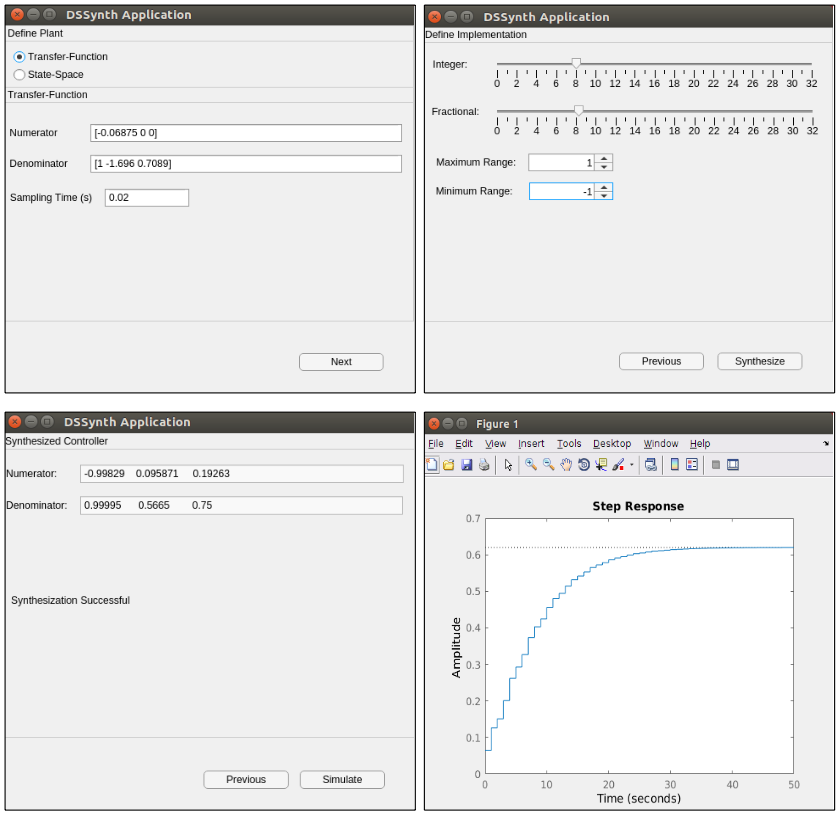
\includegraphics[width=0.5\textwidth]{screens_dssynth.png}
  \caption{GUI Application for Transfer-Function Synthesis.}
  \label{fig:gui-for-tf}
\end{figure}

%---------------------------------------------------
\subsection{Illustrative Example}
%---------------------------------------------------

To illustrate the \tool's usage, Fig.~\ref{toolbox-usage} shows the synthesis for a physical plant defined in Eq.(~\ref{equation_plant}) using the transfer-function representation, where ``num'' and ``den'' represent the numerator $A(z)$ and denominator $B(z)$, respectively.
%
\begin{equation}
\label{equation_plant}
H(z)=\frac{B(z)}{A(z)}=\frac{-0.06875z^{2}}{z^2-1.696z+0.7089},
\end{equation}
%
\begin{figure}[ht]
\scriptsize
\begin{lstlisting}[xleftmargin=.025\textwidth,xrightmargin=.025\textwidth, frame=single,]
>> num = [-0.06875 0 0];
>> den = [1.0000 -1.696 0.7089];
>> system = tf(num,den,0.002);
>> y = synthesize(system,8,8,1,-1);
>> SYNTHESIS SUCCESSFUL
>> y = (-0.9983z^2 + 0.09587z + 0.1926)/(z^2+0.5665+0.75);
\end{lstlisting}
\vspace{-0.2cm}
\caption{Synthesis of a Digital Controller for the physical plant defined in Eq.(~\ref{equation_plant}) in MATLAB, with a fixed-point format  $\left\langle 8,8\right\rangle$.}
\label{toolbox-usage}
\end{figure}
%
In the Fig.~\ref{toolbox-usage}, the value returned in $y$ represents the digital controller synthesized and stable. In order to validate and reproduce the stability in the digital system composed by the physical plant defined in Eq.(~\ref{equation_plant}) and the digital controller represented by $y$, the user can invoke the step response using the command \texttt{dstep}, and then observe that the graph plotted shows a stable digital system, as can be seen in Fig.~\ref{step-response}.
%
\begin{figure}[ht]
  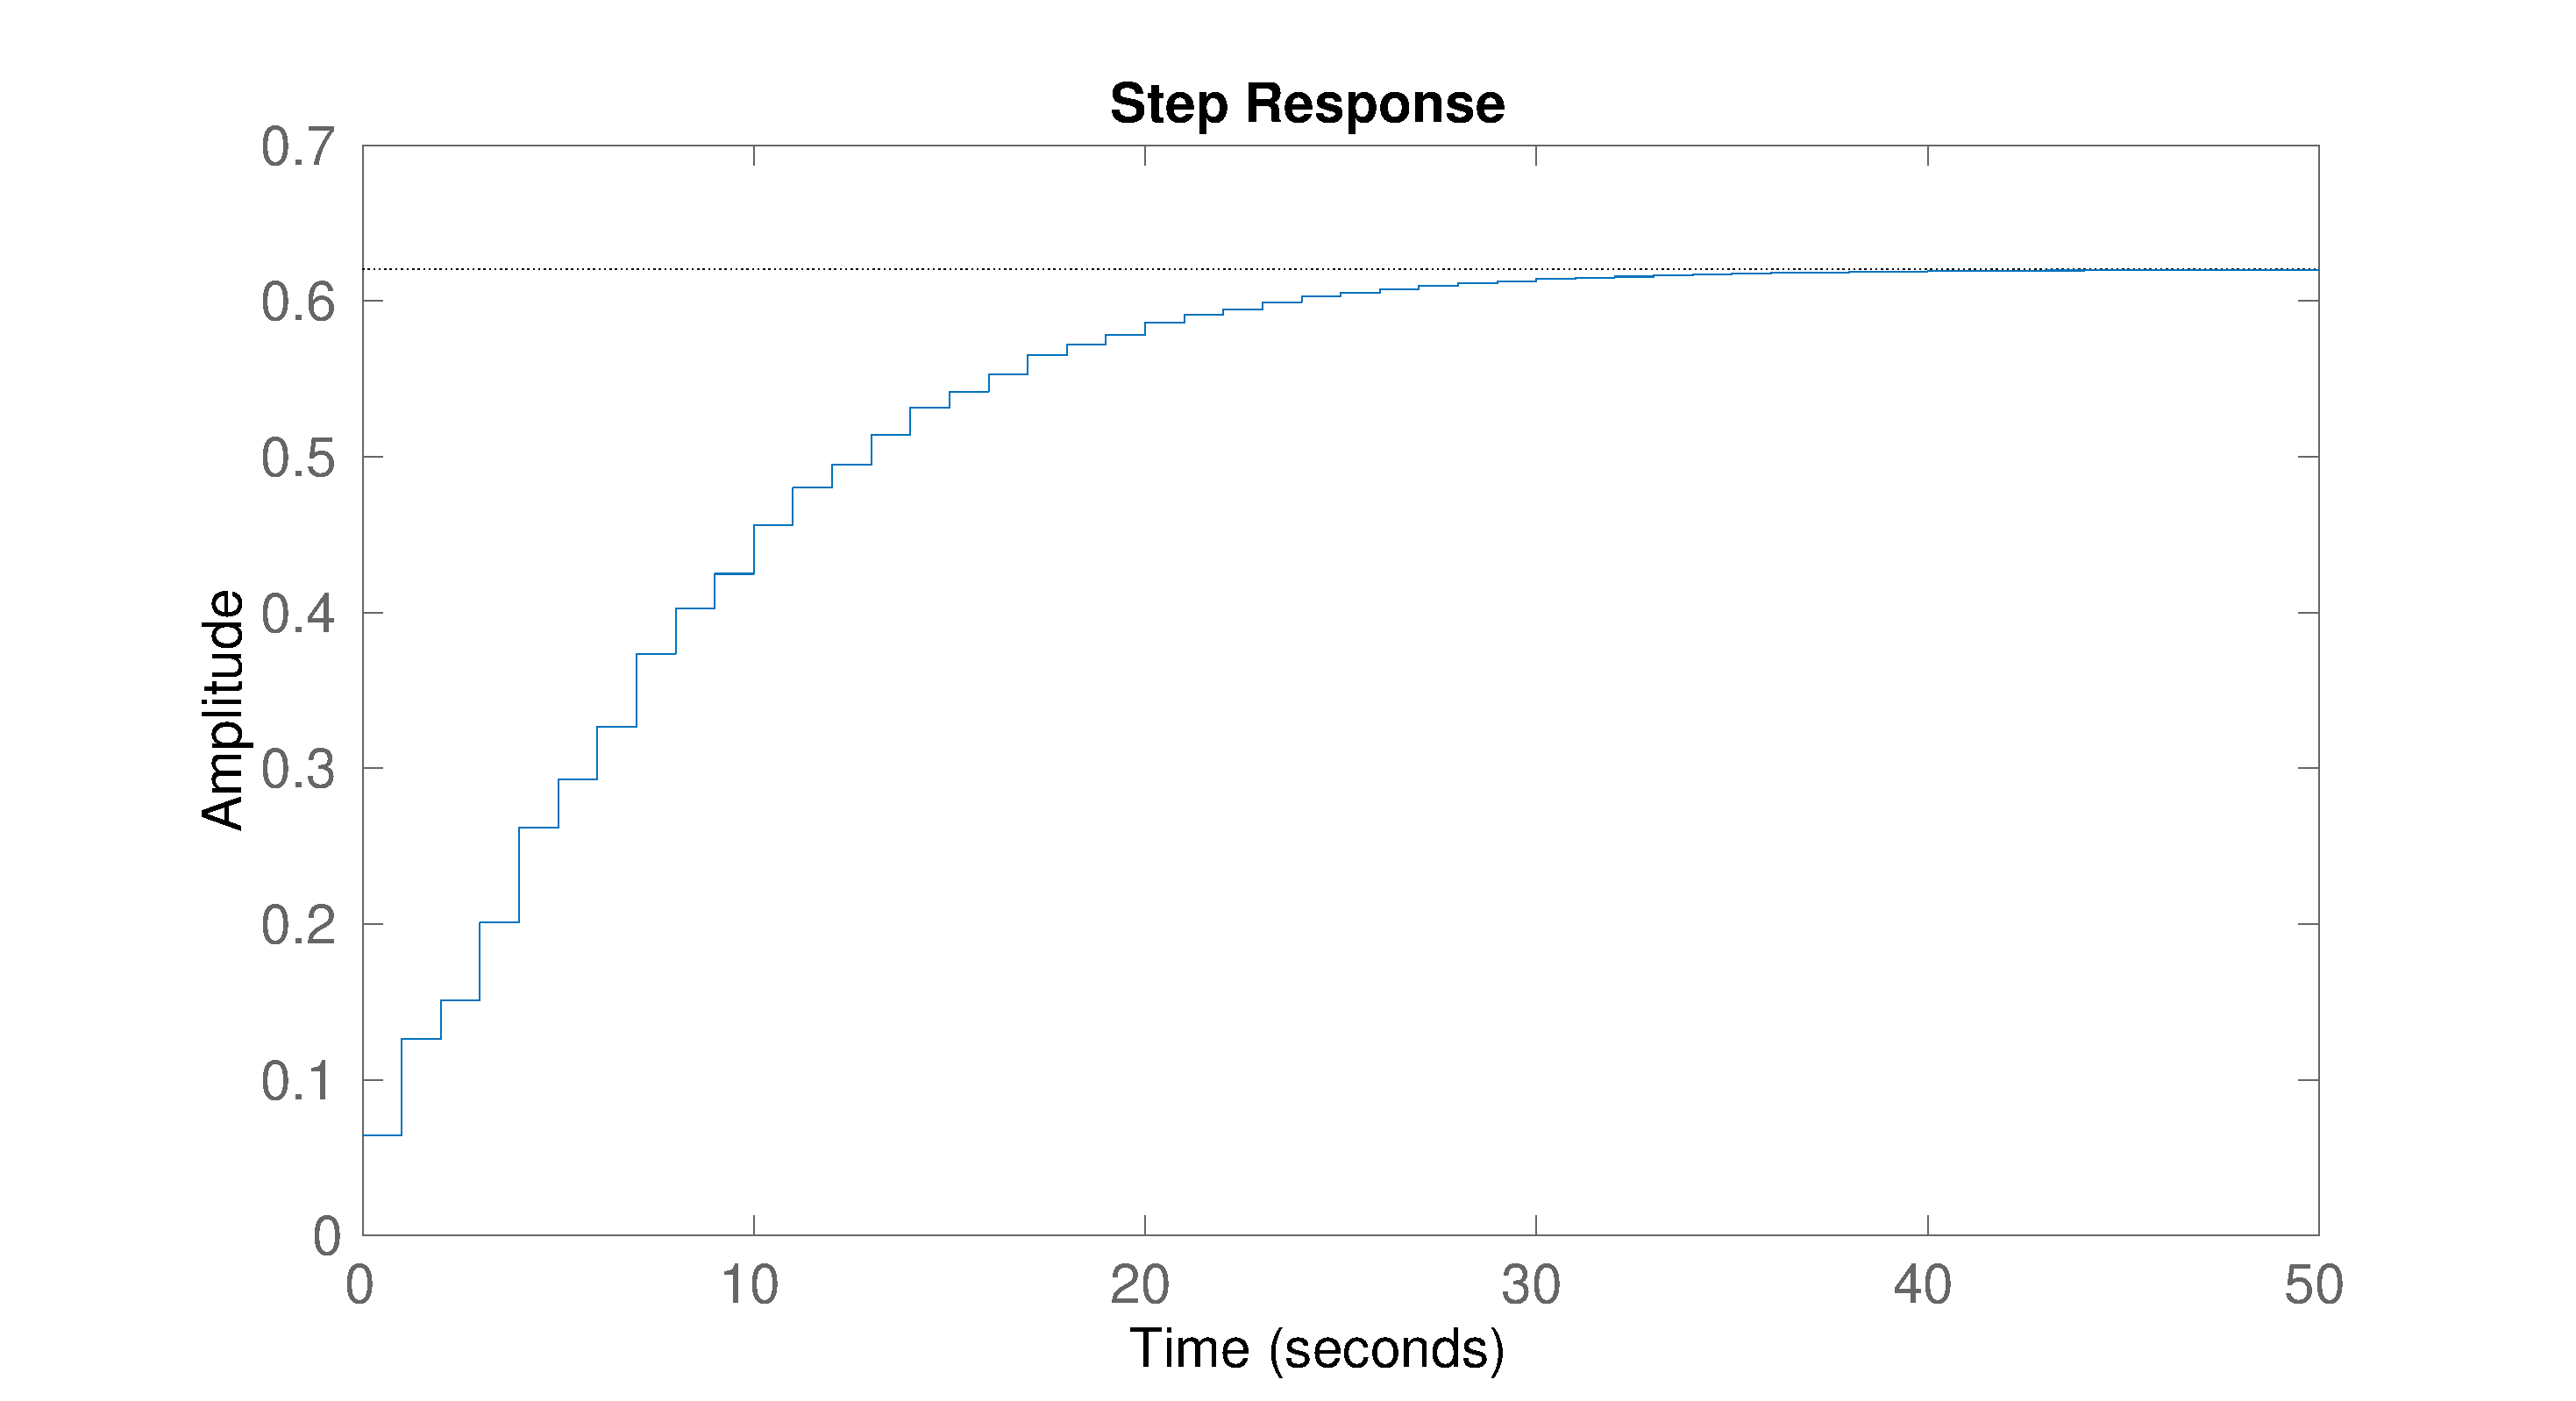
\includegraphics[width=0.5\textwidth]{step-response.eps}
  \caption{Step response for the Eq.~\eqref{equation_plant} describing a stable system.}
  \label{step-response}
\end{figure}


\section{Conclusions}

\tool is able to synthesize dynamic physical plants designed in MATLAB, through transfer-function and state-space representations based on Counter-Example Guided Inductive Synthesis (CEGIS)~\cite{DBLP:conf/asplos/Solar-LezamaTBSS06}.

Given the current literature in formal synthesis, there is no other MATLAB toolbox for synthesize stable digital systems, while taking into account implementation aspects (fixed-point arithmetic). 

As future work, \tool will perform synthesis to generate stable digital controllers and be combined with DSVerifier Toolbox~\cite{issta2017} to verify the stability of the digital controller synthesized, and also, with DSValidator Toolbox~\cite{dsvalidator}, in order to reproduce and validate the stability property.  


\bibliographystyle{ACM-Reference-Format}
\bibliography{references} 

\end{document}
